% =====================================================================
%  main.tex
%  Modul Perkuliahan Desain Web
%  Berbasis template ElegantBook (ElegantLaTeX) — desain visual dipertahankan.
%
%  Kompilasi (wajib XeLaTeX):
%    xelatex -synctex=1 -interaction=nonstopmode main.tex
%    xelatex -synctex=1 -interaction=nonstopmode main.tex   (pass kedua utk referensi)
%
%  Lihat README.md untuk instruksi lengkap.
% =====================================================================
\documentclass[lang=en, color=blue, device=normal, mode=fancy, 11pt]{elegantbook}

% --- Preamble khusus modul (bahasa Indonesia + lingkungan pedagogis) ---
% =====================================================================
%  preamble.tex
%  Preamble khusus Modul Perkuliahan Desain Web.
%
%  - Bahasa Indonesia (nama bab, gambar, tabel, dll. diterjemahkan)
%  - Palet biru/teal yang terkendali (restrained blue/teal)
%  - Lingkungan pedagogis yang dapat digunakan ulang:
%      capaian, tujuanpraktik, langkah, catatan, tip,
%      peringatan, latihan, tangkapanlayar (placeholder non-gambar)
%
%  File ini di-\input dari main.tex. Jangan kompilasi sendiri.
% =====================================================================

% ---------------------------------------------------------------------
% 1. BAHASA INDONESIA
%    ElegantBook memuat lang=en; kita terjemahkan label-label inti.
% ---------------------------------------------------------------------
\renewcommand{\chaptername}{Bab}
\renewcommand{\contentsname}{Daftar Isi}
\renewcommand{\listfigurename}{Daftar Gambar}
\renewcommand{\listtablename}{Daftar Tabel}
\renewcommand{\figurename}{Gambar}
\renewcommand{\tablename}{Tabel}
\renewcommand{\bibname}{Daftar Pustaka}
\renewcommand{\indexname}{Indeks}
\renewcommand{\appendixname}{Lampiran}
\renewcommand{\proofname}{Bukti}
\renewcommand{\notename}{Catatan}
\renewcommand{\examplename}{Contoh}
\renewcommand{\exercisename}{Latihan}
\renewcommand{\problemname}{Soal}
\renewcommand{\solutionname}{Penyelesaian}
\renewcommand{\remarkname}{Catatan}
\renewcommand{\assumptionname}{Asumsi}
\renewcommand{\conclusionname}{Kesimpulan}
\renewcommand{\propertyname}{Sifat}
\renewcommand{\introductionname}{Pendahuluan}

% ---------------------------------------------------------------------
% 2. PALET WARNA — biru/teal yang terkendali
%    ElegantBook color=blue memberi structurecolor RGB(60,113,183).
%    Kita pertajam ke biru/teal yang lebih tenang tanpa mengubah
%    arsitektur warna template (main/second/third tetap dipakai).
% ---------------------------------------------------------------------
\definecolor{structurecolor}{RGB}{38, 92, 148}   % biru utama (teal-leaning)
\definecolor{main}{RGB}{38, 92, 148}             % biru utama
\definecolor{second}{RGB}{0, 128, 128}           % teal (aksen sekunder)
\definecolor{third}{RGB}{0, 105, 148}            % biru tua (aksen tersier)

% Warna bantu untuk lingkungan pedagogis (tetap dalam keluarga biru/teal)
\definecolor{pedagogyBlue}{RGB}{38, 92, 148}
\definecolor{pedagogyTeal}{RGB}{0, 128, 128}
\definecolor{pedagogyLight}{RGB}{232, 240, 248}
\definecolor{pedagogyTealLight}{RGB}{224, 240, 240}
\definecolor{pedagogyAmber}{RGB}{176, 130, 20}   % hanya untuk peringatan (kontras)
\definecolor{pedagogyAmberLight}{RGB}{250, 244, 224}

% ---------------------------------------------------------------------
% 3. LINGKUNGAN PEDAGOGIS
%    Dibangun di atas tcolorbox (sudah dimuat ElegantBook) agar
%    konsisten dengan gaya visual template.
% ---------------------------------------------------------------------

% --- 3.1 capaian (Capaian Pembelajaran) ---
\newtcolorbox{capaian}{
  enhanced,
  breakable,
  colback=pedagogyLight,
  colframe=pedagogyBlue,
  coltitle=white,
  colbacktitle=pedagogyBlue,
  fonttitle=\bfseries,
  title={Capaian Pembelajaran},
  boxrule=0.8pt,
  arc=2pt,
  left=8pt, right=8pt, top=6pt, bottom=6pt,
  before skip=10pt, after skip=10pt
}

% --- 3.2 tujuanpraktik (Tujuan Praktik) ---
\newtcolorbox{tujuanpraktik}{
  enhanced,
  breakable,
  colback=pedagogyTealLight,
  colframe=pedagogyTeal,
  coltitle=white,
  colbacktitle=pedagogyTeal,
  fonttitle=\bfseries,
  title={Tujuan Praktik},
  boxrule=0.8pt,
  arc=2pt,
  left=8pt, right=8pt, top=6pt, bottom=6pt,
  before skip=10pt, after skip=10pt
}

% --- 3.3 langkah (Langkah Kerja) — daftar bernomor otomatis ---
\newenvironment{langkah}{%
  \par\noindent\textbf{\color{pedagogyBlue}Langkah Kerja}\par\nobreak
  \begin{enumerate}[label=\textbf{\arabic*.}, leftmargin=2em, itemsep=2pt]
}{%
  \end{enumerate}
}

% --- 3.4 catatan (Catatan) ---
\newtcolorbox{catatan}{
  enhanced,
  breakable,
  colback=pedagogyLight,
  colframe=pedagogyBlue,
  coltitle=white,
  colbacktitle=pedagogyBlue,
  fonttitle=\bfseries,
  title={Catatan},
  boxrule=0.8pt,
  arc=2pt,
  left=8pt, right=8pt, top=6pt, bottom=6pt,
  before skip=10pt, after skip=10pt
}

% --- 3.5 tip (Tips) ---
\newtcolorbox{tip}{
  enhanced,
  breakable,
  colback=pedagogyTealLight,
  colframe=pedagogyTeal,
  coltitle=white,
  colbacktitle=pedagogyTeal,
  fonttitle=\bfseries,
  title={Tips},
  boxrule=0.8pt,
  arc=2pt,
  left=8pt, right=8pt, top=6pt, bottom=6pt,
  before skip=10pt, after skip=10pt
}

% --- 3.6 peringatan (Peringatan) ---
\newtcolorbox{peringatan}{
  enhanced,
  breakable,
  colback=pedagogyAmberLight,
  colframe=pedagogyAmber,
  coltitle=white,
  colbacktitle=pedagogyAmber,
  fonttitle=\bfseries,
  title={Peringatan},
  boxrule=0.8pt,
  arc=2pt,
  left=8pt, right=8pt, top=6pt, bottom=6pt,
  before skip=10pt, after skip=10pt
}

% --- 3.7 latihan (Latihan) — wadah konten bebas (prosa, daftar, kode)
%     Digunakan bab sebagai kotak latihan; isi boleh berupa paragraf,
%     itemize/enumerate, atau lstlisting. Nomor latihan: bab.nomor.
\newcounter{latihan}[chapter]
\renewcommand{\thelatihan}{\thechapter.\arabic{latihan}}
\newenvironment{latihan}[1][]{%
  \refstepcounter{latihan}%
  \begin{tcolorbox}[
    enhanced,
    breakable,
    colback=pedagogyLight,
    colframe=pedagogyBlue,
    coltitle=white,
    colbacktitle=pedagogyBlue,
    fonttitle=\bfseries,
    title={Latihan \thelatihan~#1},
    boxrule=0.8pt,
    arc=2pt,
    left=8pt, right=8pt, top=6pt, bottom=6pt,
    before skip=10pt, after skip=10pt
  ]
}{%
  \end{tcolorbox}
}

% --- 3.8 tangkapanlayar (placeholder non-gambar)
%     Input:  #1 = jalur aset yang diharapkan (mis. assets/images/bab1/halaman-utama.png)
%             #2 = keterangan (caption)
%             #3 = instruksi untuk mahasiswa
%     Menampilkan kotak placeholder yang jelas, BUKAN gambar, sehingga
%     penulis tahu aset apa yang harus disediakan.
\NewDocumentEnvironment{tangkapanlayar}{ m m m }{%
  \begin{tcolorbox}[
    enhanced,
    breakable,
    colback=pedagogyLight,
    colframe=pedagogyBlue,
    coltitle=white,
    colbacktitle=pedagogyBlue,
    fonttitle=\bfseries,
    title={Tangkapan Layar (placeholder)},
    boxrule=0.8pt,
    arc=2pt,
    left=8pt, right=8pt, top=6pt, bottom=6pt,
    before skip=10pt, after skip=10pt
  ]
  \textbf{Jalur aset yang diharapkan:} \path{#1}\par
  \textbf{Keterangan:} #2\par
  \textbf{Instruksi mahasiswa:} #3\par
  \medskip
  \noindent\fbox{%
    \parbox{0.92\linewidth}{%
      \centering
      \vspace{1.2em}
      {\large\color{pedagogyBlue}\textbf{[ Tempatkan tangkapan layar di sini ]}}\\[0.4em]
      {\small\color{black!60}Ganti blok ini dengan \texttt{\textbackslash includegraphics} setelah aset \texttt{#1} tersedia.}
      \vspace{1.2em}
    }%
  }
}{%
  \end{tcolorbox}
}

% ---------------------------------------------------------------------
% 3.9 Definisi bahasa untuk listings (css & javascript)
%     Listings di TeX Live ini tidak memuat bahasa css/javascript secara
%     bawaan; didefinisikan di sini agar blok kode bab dapat dikompilasi.
% ---------------------------------------------------------------------
\lstdefinelanguage{css}{
  morekeywords={color,background,background-color,background-image,border,
    border-radius,box-shadow,display,flex,flex-direction,flex-wrap,justify-content,
    align-items,gap,grid,grid-template-columns,grid-template-rows,grid-gap,
    margin,padding,width,height,max-width,min-width,font,font-family,font-size,
    font-weight,text-align,text-decoration,line-height,position,top,right,bottom,
    left,z-index,overflow,opacity,transition,transform,animation,media,float,
    clear,list-style,content,cursor,visibility,vertical-align,white-space},
  sensitive=true,
  morecomment=[l]{//},
  morecomment=[s]{/*}{*/},
  morestring=[b]',
  morestring=[b]"
}

\lstdefinelanguage{JavaScript}{
  keywords={break,case,catch,class,const,continue,debugger,default,delete,do,
    else,export,extends,finally,for,function,if,import,in,instanceof,let,new,
    return,super,switch,this,throw,try,typeof,var,void,while,with,yield,async,
    await,of,static,get,set,true,false,null,undefined},
  sensitive=true,
  morecomment=[l]{//},
  morecomment=[s]{/*}{*/},
  morestring=[b]',
  morestring=[b]"
}

% ---------------------------------------------------------------------
% 4. KONVENSI ASET
%    Jalur relatif terhadap folder book/.
%    - Gambar:  assets/images/<bab>/<nama>.png
%    - Kode:    assets/code/<bab>/<nama>.html
%    Gunakan \figref{label} (disediakan ElegantBook) untuk referensi.
% ---------------------------------------------------------------------
\graphicspath{{assets/images/}}

% ---------------------------------------------------------------------
% 5. HIPERLINK — warna tautan mengikuti palet biru/teal
% ---------------------------------------------------------------------
\hypersetup{
  colorlinks=true,
  linkcolor=pedagogyBlue,
  citecolor=pedagogyTeal,
  urlcolor=pedagogyTeal
}


% =====================================================================
%  METADATA BUKU
% =====================================================================
\title{Modul Perkuliahan Desain Web}
\subtitle{Panduan Praktik dan Latihan Terstruktur}
\author{Raksa Zhidane Nashrul Huda}
\institute{D3 Teknik Informaatika}
\date{\today}
\version{1.0}
\bioinfo{Penggunaan}{Untuk kalangan mahasiswa}

% =====================================================================
%  DOKUMEN
% =====================================================================
\begin{document}

\maketitle

\frontmatter
\tableofcontents
\listoffigures
\listoftables

\mainmatter

% --- Bab-bab modul (minggu 01–16) ---
% =====================================================================
%  chapters/minggu-01.tex
%  Minggu 1 — Pengantar Web \& Setup Lingkungan Kerja
% =====================================================================

\chapter{Pengantar Web \& Setup Lingkungan Kerja}
\label{chap:minggu-01}

% ---------------------------------------------------------------------
% 1. CAPAIAN PEMBELAJARAN
% ---------------------------------------------------------------------
\begin{capaian}
Setelah menyelesaikan bab ini, mahasiswa diharapkan mampu:
\begin{itemize}
  \item menjelaskan alur kerja \emph{design-to-code} dalam pengembangan web;
  \item menginstal dan mengonfigurasi VS Code beserta ekstensi yang diperlukan;
  \item membuat akun GitHub dan melakukan \emph{push} pertama ke \emph{repository};
  \item membuka file HTML di peramban menggunakan \emph{Live Server}.
\end{itemize}
\end{capaian}

% ---------------------------------------------------------------------
% 2. TUJUAN PRAKTIK
% ---------------------------------------------------------------------
\begin{tujuanpraktik}
Pada sesi praktik ini, mahasiswa akan:
\begin{itemize}
  \item menginstal VS Code dan ekstensi pendukung;
  \item membuat file HTML pertama dan melihat hasilnya di peramban;
  \item membuat akun GitHub serta \emph{repository} pertama;
  \item melakukan \emph{push} kode ke GitHub.
\end{itemize}
\end{tujuanpraktik}

% ---------------------------------------------------------------------
% 3. PENGANTAR: APA ITU WEB?
% ---------------------------------------------------------------------
\section{Pengenalan Web}
\label{sec:m01-pengenalan}

Website adalah kumpulan halaman yang diakses melalui peramban (\emph{browser}) seperti Chrome, Firefox, atau Edge. Setiap halaman web terdiri dari tiga lapis utama:

\begin{table}[ht]
\centering
\caption{Tiga lapis utama halaman web}
\label{tab:m01-lapis}
\begin{tabular}{llp{7cm}}
\toprule
\textbf{Lapis} & \textbf{Bahasa} & \textbf{Fungsi} \\
\midrule
Struktur & HTML & ``Tulang'' — menentukan elemen apa yang ada di halaman \\
Tampilan & CSS & ``Kulit'' — menentukan warna, ukuran, posisi, font \\
Interaksi & JavaScript & ``Otot'' — menentukan apa yang terjadi saat diklik/di-scroll \\
\bottomrule
\end{tabular}
\end{table}

\begin{catatan}
Mahasiswa tidak perlu menghafal ketiga lapis ini sekarang. Cukup ketahui bahwa ada tiga lapis; di minggu-minggu berikutnya kita akan pelajari satu per satu.
\end{catatan}

% ---------------------------------------------------------------------
% 4. ALUR KERJA DESIGN-TO-CODE
% ---------------------------------------------------------------------
\section{Alur Kerja \emph{Design-to-Code}}
\label{sec:m01-alur}

Alur kerja pengembangan web mengikuti urutan berikut:

\begin{enumerate}
  \item \textbf{Ide / Kebutuhan} — menentukan tujuan dan isi halaman.
  \item \textbf{Figma} — mendesain tampilan visual.
  \item \textbf{VS Code} — menulis kode HTML, CSS, dan JavaScript.
  \item \textbf{Peramban} — melihat dan menguji hasil.
  \item \textbf{GitHub} — menyimpan kode agar bisa diakses kapan saja.
\end{enumerate}

Intinya: desain di Figma\,$\rightarrow$\,implementasi di VS Code\,$\rightarrow$\,lihat hasil di peramban\,$\rightarrow$\,simpan di GitHub.

% ---------------------------------------------------------------------
% 5. LIVE CODING: INSTALASI VS CODE \& EKSTENSI
% ---------------------------------------------------------------------
\section{Instalasi VS Code \& Ekstensi}
\label{sec:m01-instalasi}

\subsection{Download \& Instal VS Code}

\begin{langkah}
  \item Buka peramban, kunjungi \texttt{https://code.visualstudio.com/}.
  \item Klik tombol \textbf{Download for Windows} (atau sesuai OS).
  \item Jalankan installer, klik \textbf{Next} di setiap langkah, pastikan opsi berikut diceklis:
  \begin{itemize}
    \item Add ``Open with Code'' action to Windows Explorer file context menu
    \item Add ``Open with Code'' action to Windows Explorer directory context menu
    \item Register Code as an editor for supported file types
  \end{itemize}
  \item Klik \textbf{Install}, tunggu selesai, lalu klik \textbf{Finish}.
\end{langkah}

\subsection{Instal Ekstensi Penting}

Buka VS Code, tekan \textbf{Ctrl + Shift + X} untuk membuka panel \emph{Extensions}. Cari dan instal ekstensi berikut:

\begin{table}[ht]
\centering
\caption{Ekstensi VS Code yang diperlukan}
\label{tab:m01-ekstensi}
\begin{tabular}{llp{6cm}}
\toprule
\textbf{No.} & \textbf{Nama Ekstensi} & \textbf{Fungsi} \\
\midrule
1 & Live Server (Ritwick Dey) & Preview halaman HTML otomatis di peramban saat file disimpan \\
2 & HTML CSS Support & Autocomplete kelas CSS di file HTML \\
3 & Prettier -- Code formatter & Format kode otomatis agar rapi \\
4 & VS Code Intellicode & Saran kode cerdas dari AI \\
\bottomrule
\end{tabular}
\end{table}

\subsection{Verifikasi Instalasi}

\begin{langkah}
  \item Buka VS Code.
  \item Buat folder baru: \textbf{File\,$\rightarrow$\,Open Folder\,$\rightarrow$\,New Folder}, beri nama \texttt{latihan-web-1}.
  \item Di dalam folder itu, buat file baru bernama \texttt{index.html}.
  \item Ketik \texttt{!} lalu tekan \textbf{Tab} — VS Code akan mengisi template HTML secara otomatis (\emph{snippets} Emmet).
  \item Ubah isi \texttt{<title>} menjadi \texttt{Halo Dunia}.
  \item Tambahkan di dalam \texttt{<body>}:
\end{langkah}

\begin{lstlisting}[language=HTML, caption={Kode ``Halo Dunia''}, label={lst:m01-halo}]
<h1>Halo, Dunia!</h1>
<p>Ini halaman web pertamaku.</p>
\end{lstlisting}

\begin{langkah}
  \item Klik kanan di editor $\rightarrow$ \textbf{Open with Live Server}.
  \item Peramban akan terbuka secara otomatis menampilkan teks ``Halo, Dunia!''.
\end{langkah}

\begin{figure}[htbp]
  \centering
  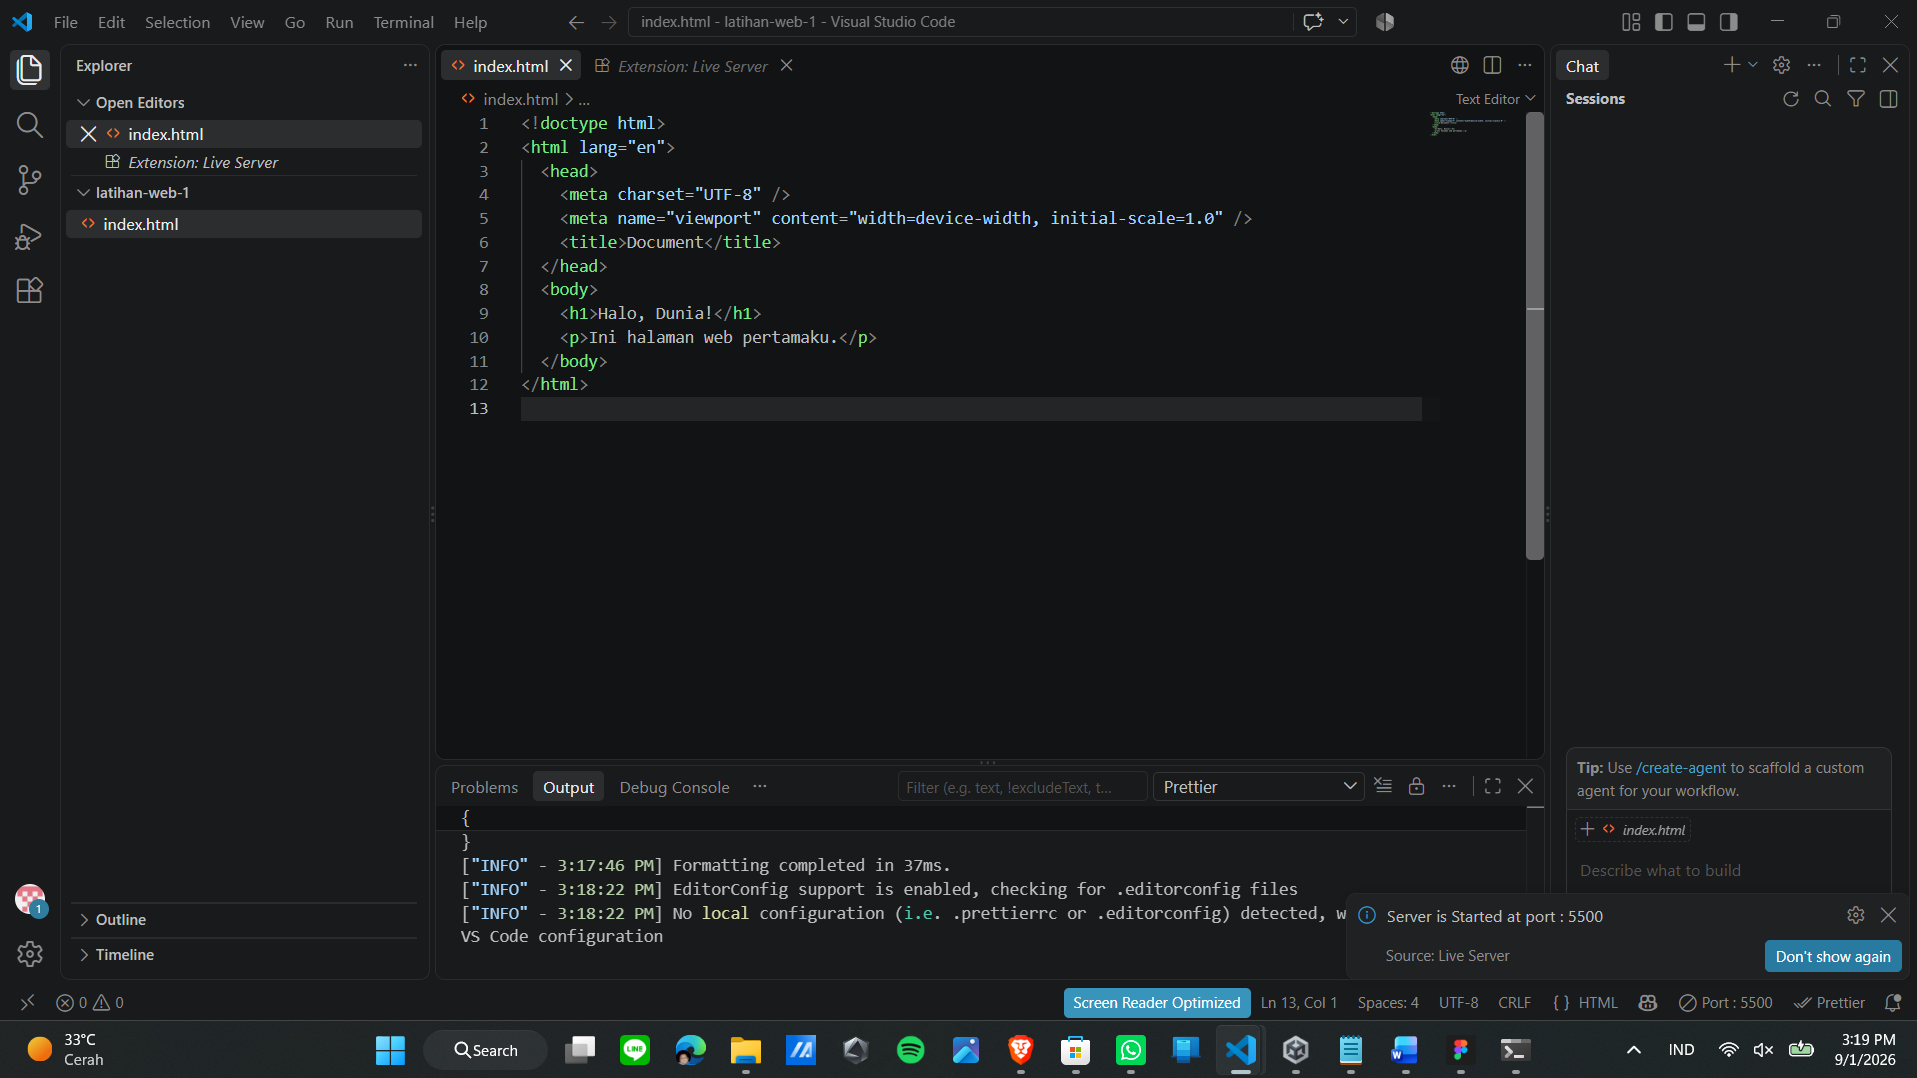
\includegraphics[width=0.85\linewidth]{minggu-01/vs-code-index.html.png}
  \caption{VS Code dengan file \texttt{index.html} terbuka.}
  \label{fig:vs-code-index}
\end{figure}

\begin{figure}[htbp]
  \centering
  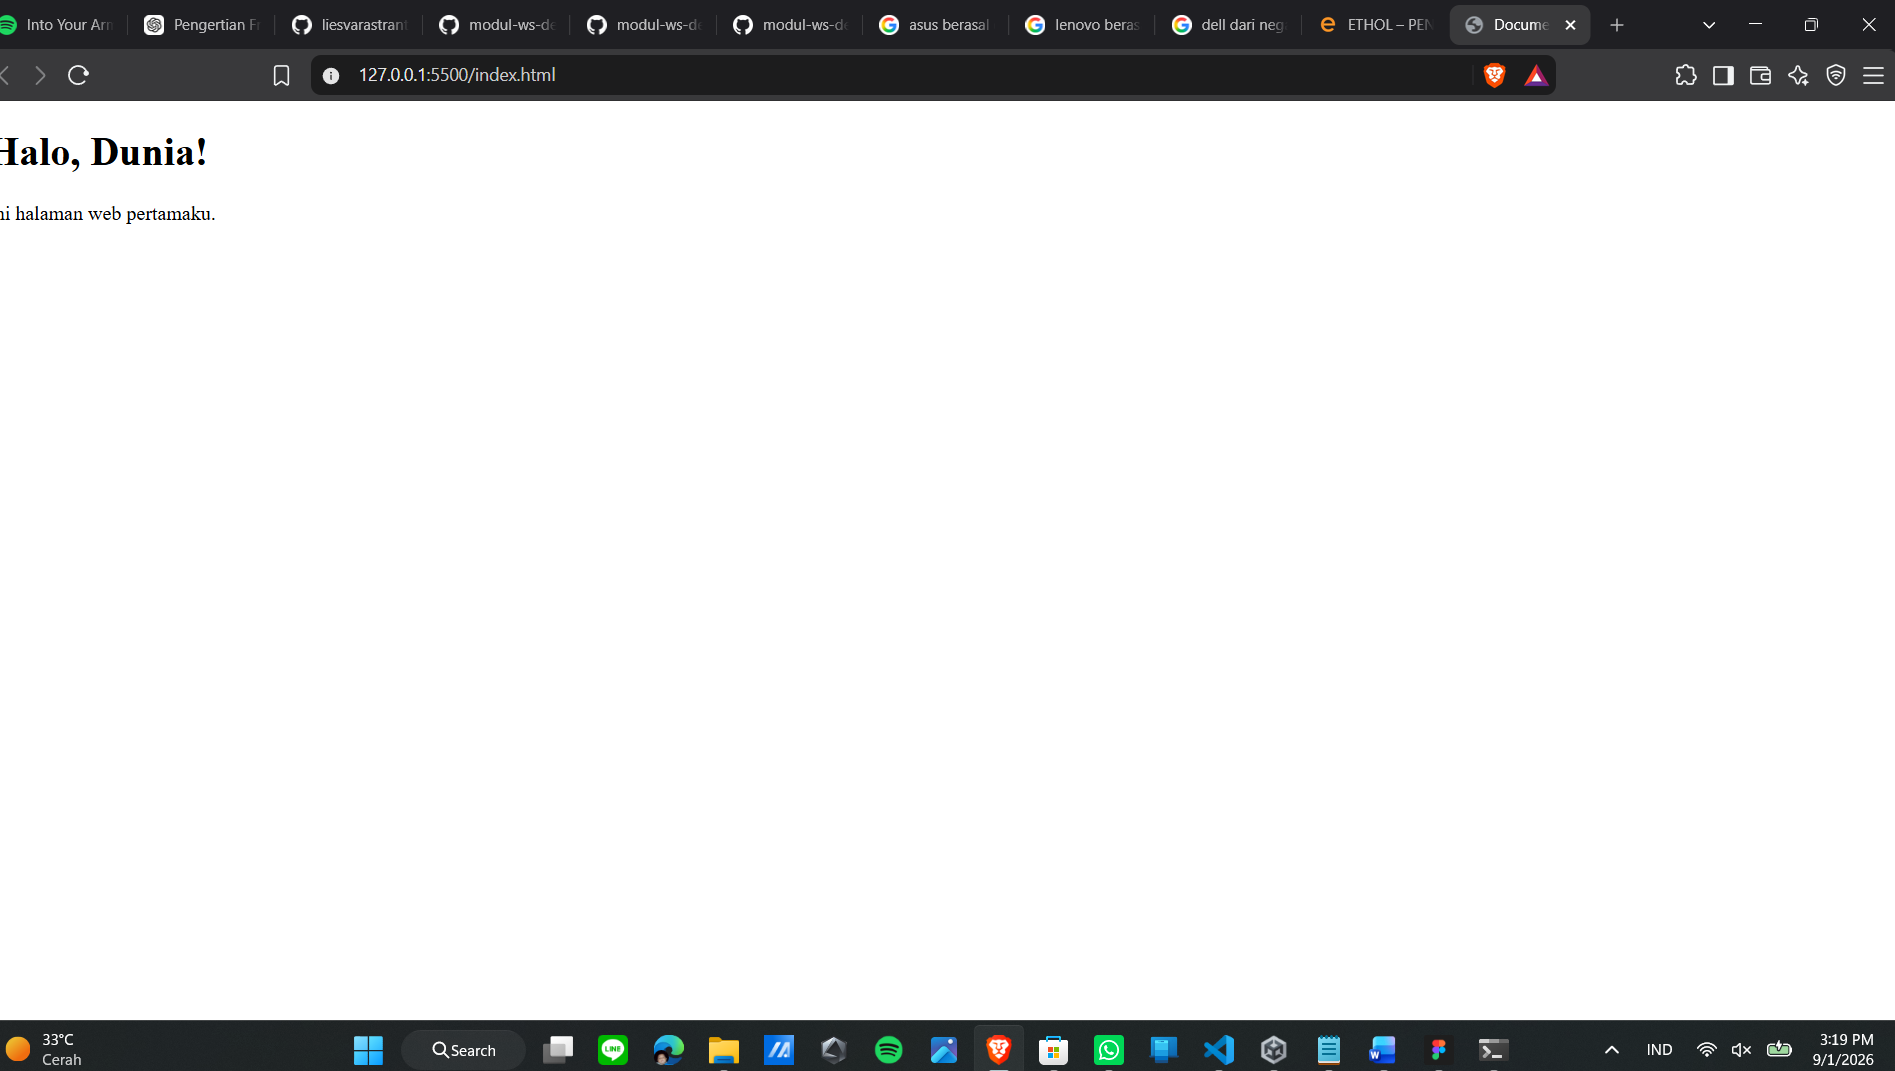
\includegraphics[width=0.85\linewidth]{minggu-01/browser-halo-dunia.png}
  \caption{Peramban menampilkan hasil ``Halo, Dunia!''}
  \label{fig:browser-halo-dunia}
\end{figure}

% ---------------------------------------------------------------------
% 6. LIVE CODING: AKUN GITHUB \& REPOSITORY PERTAMA
% ---------------------------------------------------------------------
\section{Akun GitHub \& Repository Pertama}
\label{sec:m01-github}

\subsection{Buat Akun GitHub}

\begin{langkah}
  \item Buka \texttt{https://github.com}.
  \item Klik \textbf{Sign up}.
  \item Isi email, password, dan username (gunakan format: \texttt{nama-nim}, misal: \texttt{budi-2301001}).
  \item Selesaikan verifikasi.
\end{langkah}

\begin{figure}[htbp]
  \centering
  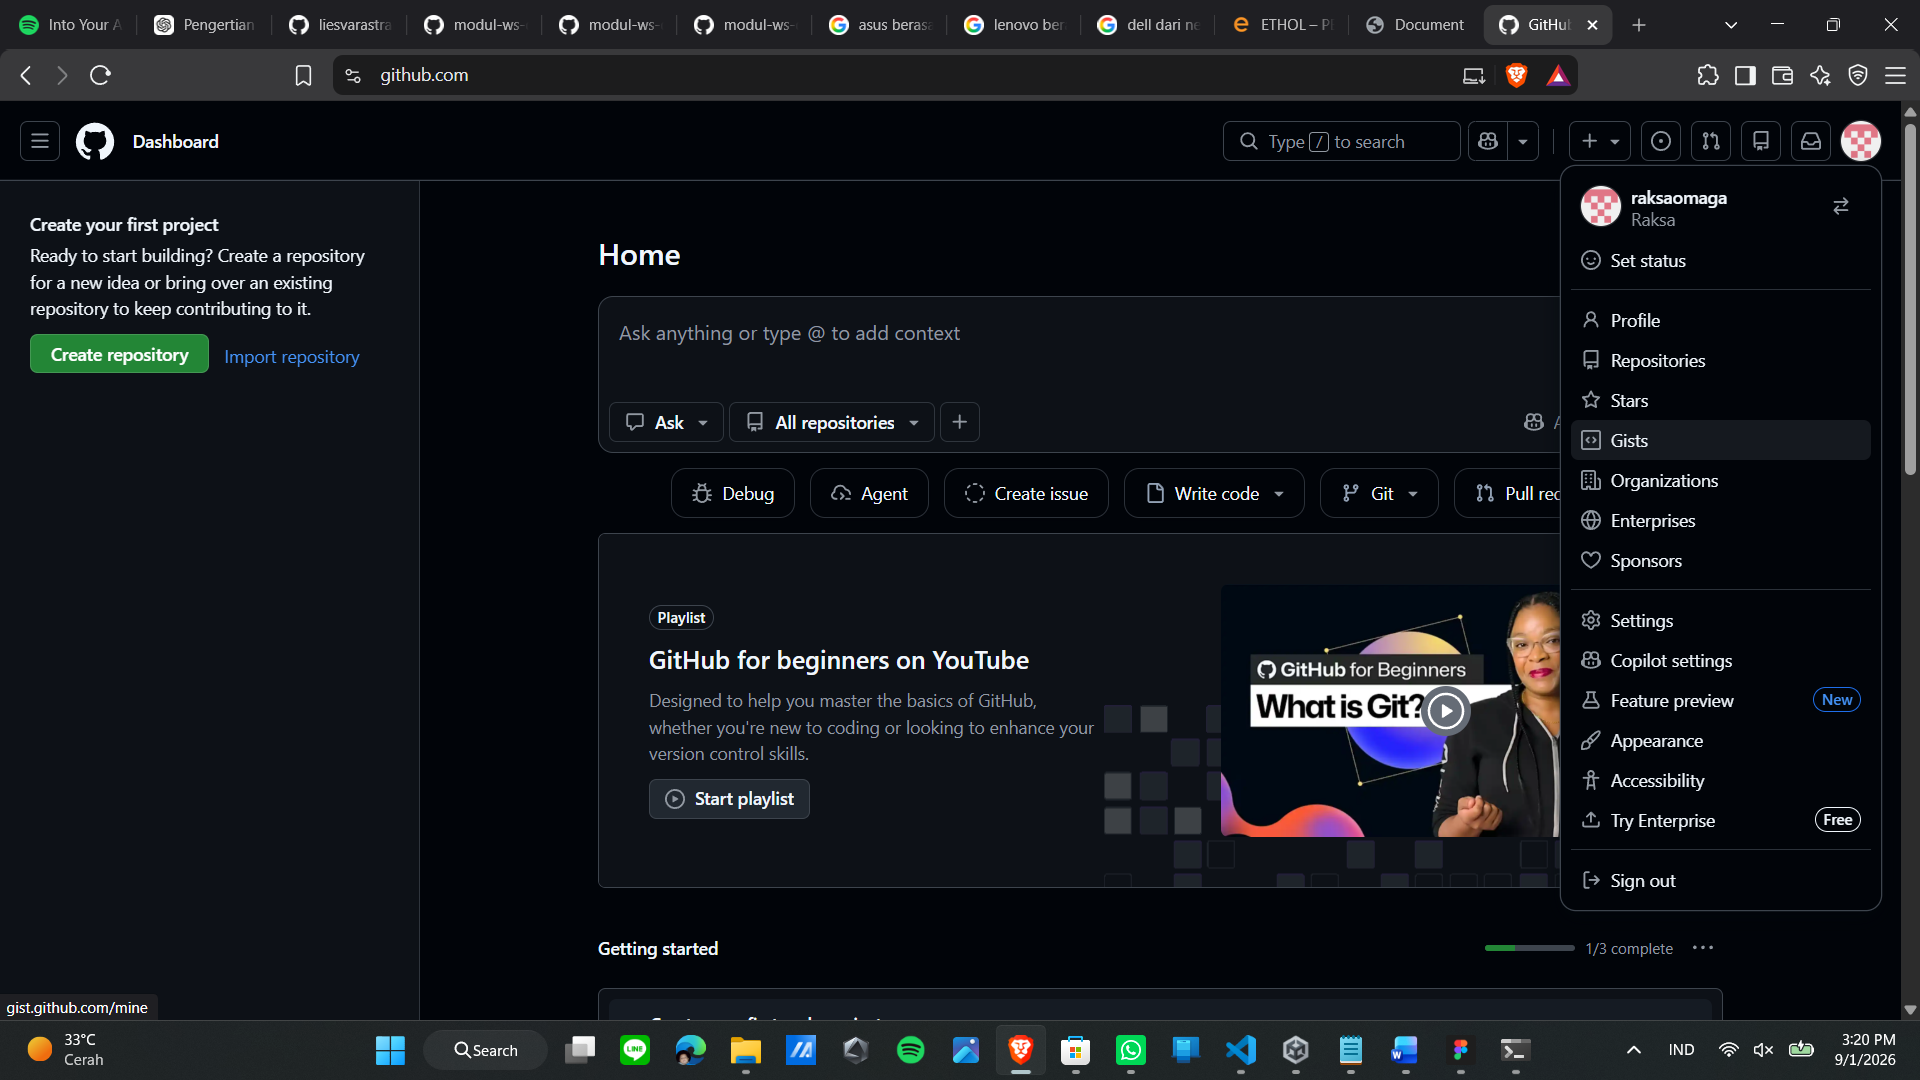
\includegraphics[width=0.85\linewidth]{minggu-01/dashboard-github.png}
  \caption{Dashboard GitHub setelah berhasil login.}
  \label{fig:dashboard-github}
\end{figure}

\subsection{Buat Repository Baru}

\begin{langkah}
  \item Di dashboard GitHub, klik tombol \textbf{+} (pojok kanan atas) $\rightarrow$ \textbf{New repository}.
  \item Isi form berikut:
  \begin{itemize}
    \item \textbf{Repository name:} \texttt{latihan-web-1}
    \item \textbf{Description:} \texttt{Latihan pertama --- Halo Dunia}
    \item Pilih \textbf{Public}
    \item Centang \textbf{Add a README file}
  \end{itemize}
  \item Klik \textbf{Create repository}.
\end{langkah}

\subsection{Hubungkan Folder Lokal ke GitHub (\emph{Push} Pertama)}

\begin{peringatan}
Pastikan Git sudah terinstal di laptop. Jika belum, unduh dari \texttt{https://git-scm.com/download/win} dan instal dengan pengaturan default.
\end{peringatan}

Buka \textbf{Terminal} di VS Code (\textbf{Ctrl + \$} atau menu \textbf{Terminal\,$\rightarrow$\,New Terminal}), lalu ketik perintah berikut satu per satu:

\begin{lstlisting}[language=bash, caption={Perintah push pertama ke GitHub}, label={lst:m01-git-push}]
# 1. Inisialisasi Git di folder lokal
git init

# 2. Hubungkan ke remote repository
#    (ganti NAMA_USER dengan username GitHub-mu)
git remote add origin https://github.com/NAMA_USER/latihan-web-1.git

# 3. Tambahkan semua file untuk di-commit
git add .

# 4. Buat commit pertama
git commit -m "Commit pertama: Halo Dunia"

# 5. Push ke GitHub
git branch -M main
git push -u origin main
\end{lstlisting}

\begin{catatan}
Jika Git meminta \emph{credential} (username \& password), gunakan \textbf{Personal Access Token} sebagai password:
\begin{enumerate}
  \item Buka \texttt{https://github.com/settings/tokens}.
  \item Klik \textbf{Generate new token (classic)}.
  \item Beri nama token, centang \textbf{repo}, lalu klik \textbf{Generate}.
  \item Salin token dan gunakan sebagai password saat Git meminta.
\end{enumerate}
\end{catatan}

\subsection{Verifikasi}

Buka \texttt{https://github.com/NAMA\_USER/latihan-web-1} di peramban. Pastikan file \texttt{index.html} terlihat di daftar file.

\begin{figure}[htbp]
  \centering
  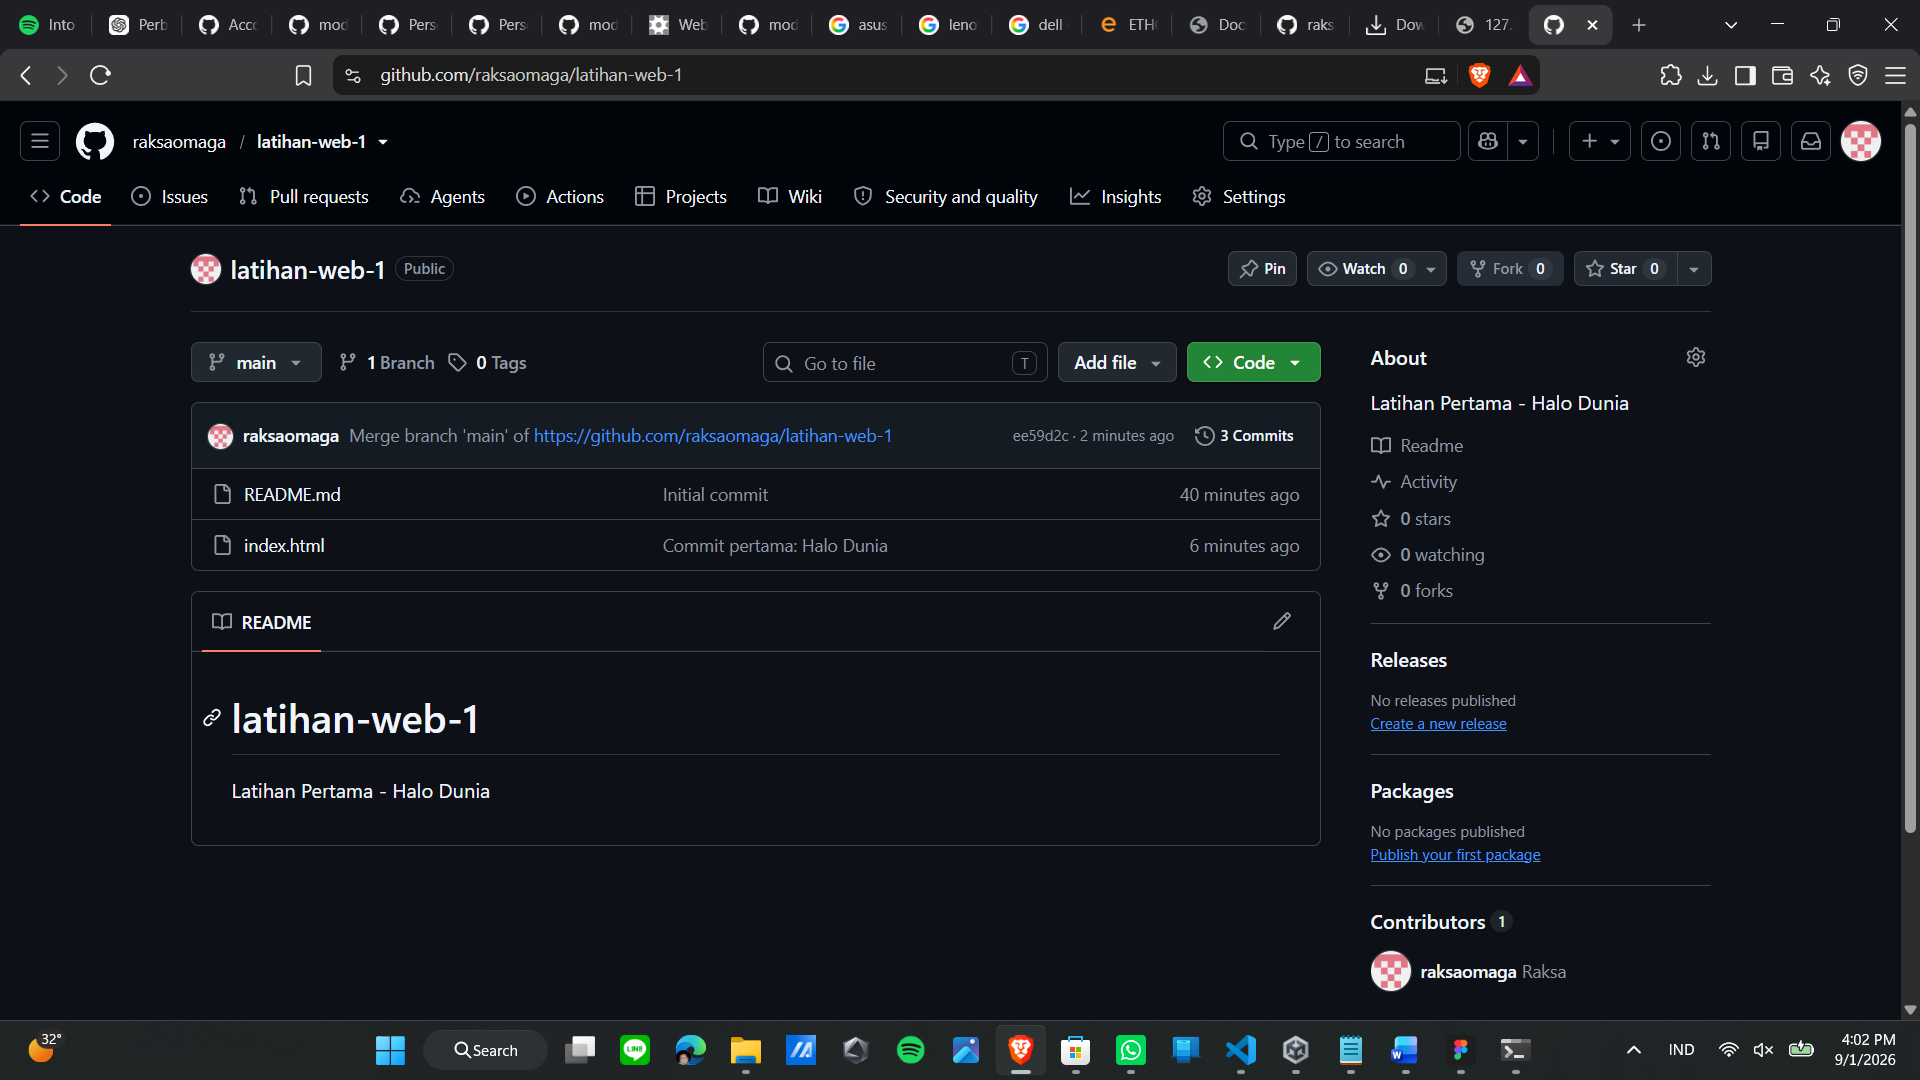
\includegraphics[width=0.85\linewidth]{minggu-01/repository-github.png}
  \caption{Halaman repository GitHub \texttt{latihan-web-1}.}
  \label{fig:repository-github}
\end{figure}

% ---------------------------------------------------------------------
% 7. LATIHAN MANDIRI
% ---------------------------------------------------------------------
\section{Latihan Mandiri}
\label{sec:m01-latihan}

\begin{latihan}[Perbarui Halaman]
Buka file \texttt{index.html} di VS Code. Tambahkan elemen berikut di bawah \texttt{<p>} yang sudah ada:
\begin{lstlisting}[language=HTML]
<h2>Tentang Aku</h2>
<p>Nama: [nama lengkap kamu]</p>
<p>NIM: [NIM kamu]</p>
<p>Prodi: D3 Informatika</p>
\end{lstlisting}
Simpan file (\textbf{Ctrl + S}), periksa peramban, lalu \emph{commit} dan \emph{push} perubahan ke GitHub.
\end{latihan}

\begin{latihan}[Eksperimen \emph{Live Server}]
\begin{enumerate}
  \item Matikan \emph{Live Server} (klik \textbf{Port: 5500\,$\rightarrow$\,Stop} di pojok kanan bawah VS Code).
  \item Buka file \texttt{index.html} langsung dari File Explorer (klik ganda).
  \item Perhatikan URL di peramban --- apakah berbeda dari URL \emph{Live Server}? (\texttt{file:///...} vs \texttt{127.0.0.1:5500})
  \item Ubah salah satu teks di VS Code $\rightarrow$ simpan $\rightarrow$ muat ulang peramban secara manual.
  \item Aktifkan kembali \emph{Live Server}. Ubah teks lagi $\rightarrow$ simpan $\rightarrow$ perhatikan apakah peramban memperbarui diri secara otomatis.
\end{enumerate}
\end{latihan}

\begin{figure}[htbp]
  \centering
  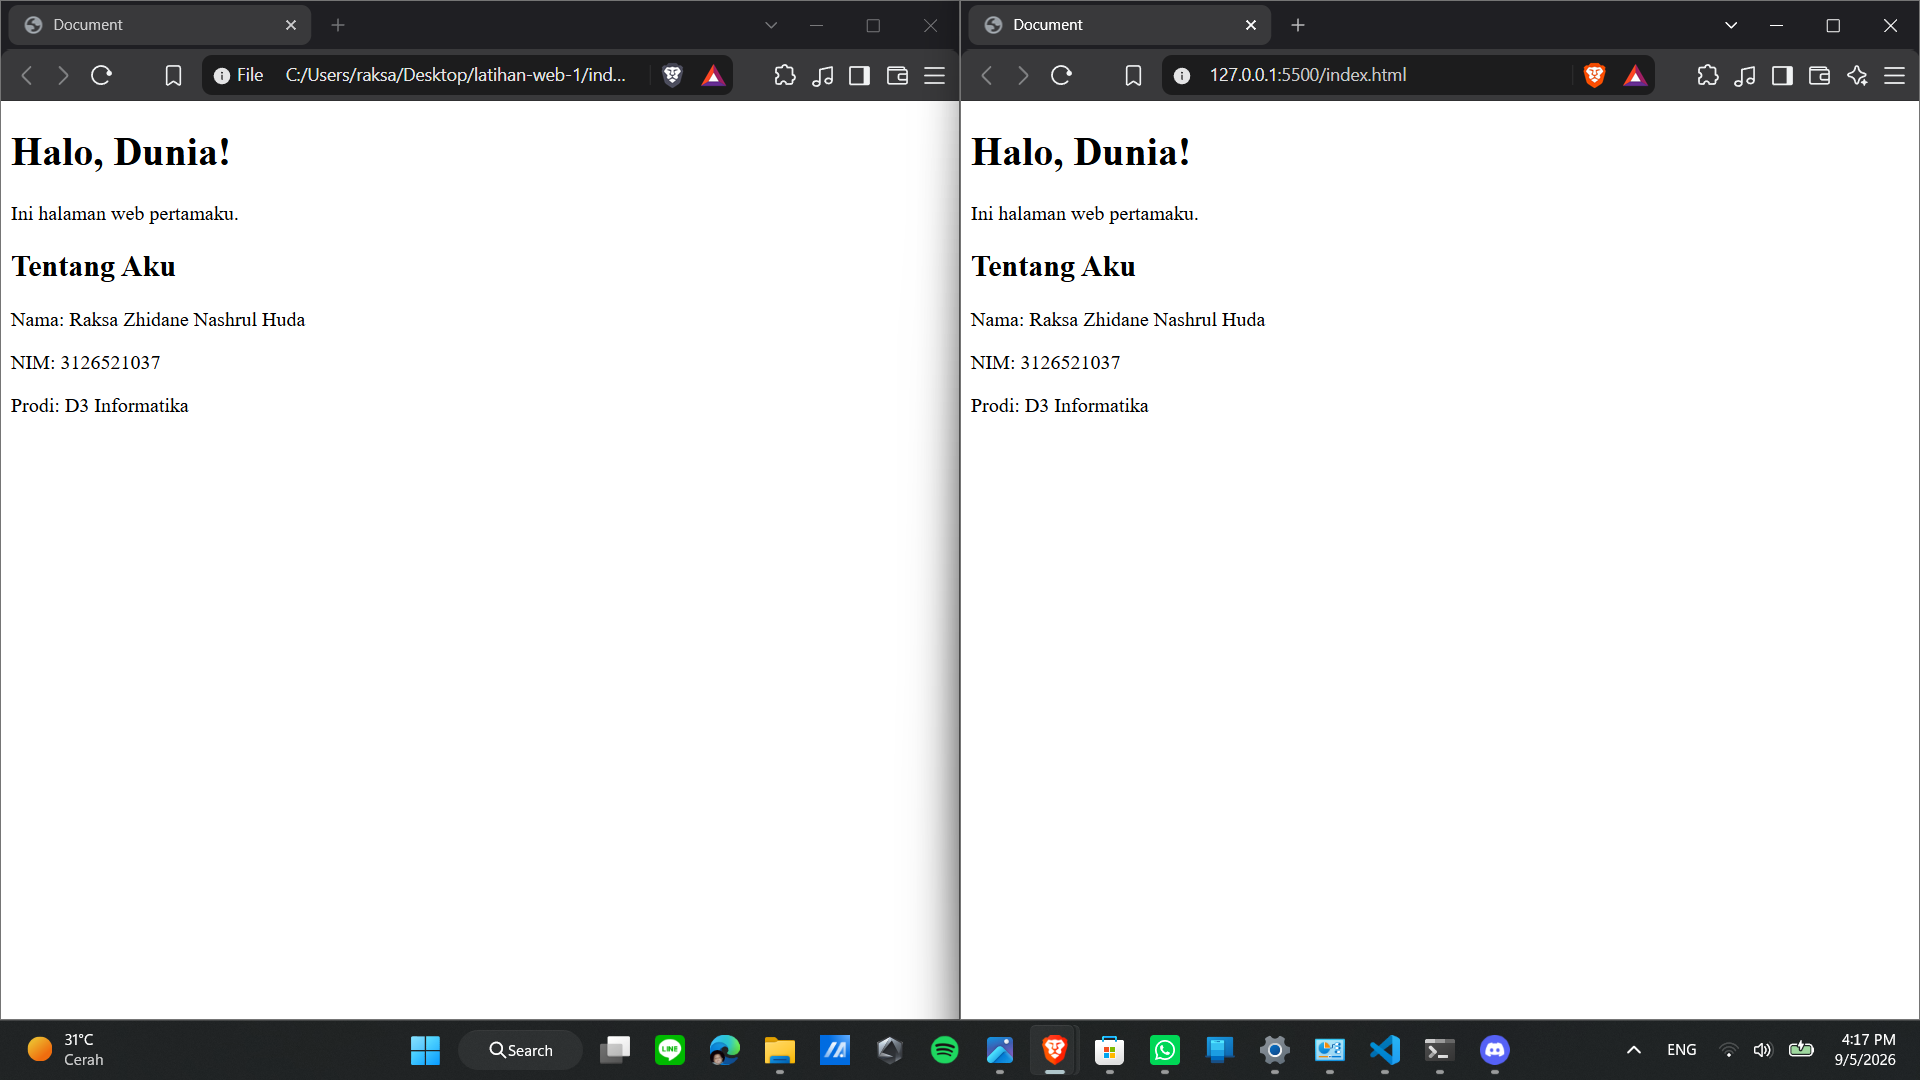
\includegraphics[width=0.85\linewidth]{minggu-01/perbandingan-url.png}
  {Perbandingan URL: \emph{Live Server} vs file langsung.}
  {Kiri: \texttt{127.0.0.1:5500/index.html}; kanan: \texttt{file:///C:/.../index.html}.}
\end{figure}

% ---------------------------------------------------------------------
% 8. TROUBLESHOOTING
% ---------------------------------------------------------------------
\section{Troubleshooting}
\label{sec:m01-troubleshoot}

\begin{table}[ht]
\centering
\caption{Masalah umum dan solusinya}
\label{tab:m01-troubleshoot}
\small
\begin{tabular}{p{4.5cm}p{8cm}}
\toprule
\textbf{Masalah} & \textbf{Solusi} \\
\midrule
\emph{Live Server} tidak muncul di menu kanan-klik & Pastikan ekstensi ``Live Server'' sudah terinstal dan VS Code di-\emph{restart} \\
Peramban menampilkan \texttt{This site can't be reached} & Pastikan \emph{Live Server} sudah berjalan (lihat \emph{status bar} pojok kanan bawah VS Code) \\
Git menolak \emph{push} karena ``repository not found'' & Periksa URL \emph{remote}: \texttt{git remote -v}, lalu perbaiki dengan \texttt{git remote set-url origin URL\_BARU} \\
Git meminta \emph{password} tapi tidak bisa login & Gunakan \textbf{Personal Access Token} (bukan \emph{password} GitHub biasa) \\
VS Code menampilkan error ``command not found: git'' & Instal Git dari \texttt{https://git-scm.com/download/win}, lalu \emph{restart} VS Code \\
File \texttt{index.html} tidak muncul di GitHub & Pastikan sudah menjalankan \texttt{git add .}, \texttt{git commit}, dan \texttt{git push} \\
\bottomrule
\end{tabular}
\end{table}

% ---------------------------------------------------------------------
% 9. RANGKUMAN
% ---------------------------------------------------------------------
\section{Rangkuman}
\label{sec:m01-rangkuman}

\begin{itemize}
  \item Alur kerja \emph{design-to-code}: Figma $\rightarrow$ VS Code $\rightarrow$ Peramban $\rightarrow$ GitHub.
  \item VS Code + ekstensi (\emph{Live Server}, Prettier, dll.) sudah terinstal.
  \item File HTML pertama berhasil dibuat dan dilihat di peramban.
  \item Akun GitHub dan \emph{repository} pertama sudah dibuat.
  \item \emph{Push} pertama ke GitHub berhasil dilakukan.
  \item \emph{Live Server} memberikan \emph{preview} otomatis tanpa \emph{reload}.
\end{itemize}

% =====================================================================
%  chapters/minggu-02.tex
%  Minggu 2 — Figma Dasar & Pengantar UI/UX
% =====================================================================

\chapter{Figma Dasar \& Pengantar UI/UX}
\label{chap:minggu-02}

% ---------------------------------------------------------------------
% 1. CAPAIAN PEMBELAJARAN
% ---------------------------------------------------------------------
\begin{capaian}
Setelah menyelesaikan bab ini, mahasiswa diharapkan mampu:
\begin{itemize}
  \item mengoperasikan antarmuka dasar Figma (frame, shape, text, layers);
  \item membuat wireframe sederhana untuk satu halaman web;
  \item menjelaskan tiga konsep dasar UI/UX: heuristik, hierarchy, dan aksesibilitas;
  \item menerapkan konsep UI/UX ke dalam desain wireframe.
\end{itemize}
\end{capaian}

% ---------------------------------------------------------------------
% 2. TUJUAN PRAKTIK
% ---------------------------------------------------------------------
\begin{tujuanpraktik}
Pada sesi praktik ini, mahasiswa akan:
\begin{itemize}
  \item mengenal antarmuka dan alat dasar Figma;
  \item membuat wireframe halaman ``Profil Diri'' untuk perangkat \emph{mobile};
  \item mempelajari tiga konsep UI/UX dan menerapkannya pada wireframe.
\end{itemize}
\end{tujuanpraktik}

% ---------------------------------------------------------------------
% 3. LIVE CODING: PENGENALAN FIGMA
% ---------------------------------------------------------------------
\section{Pengenalan Figma}
\label{sec:m02-figma}

\subsection{Akses Figma}

\begin{langkah}
  \item Buka \texttt{https://www.figma.com} di peramban.
  \item Klik \textbf{Log in}, masuk dengan akun yang sudah dibuat (atau daftar jika belum).
  \item Kamu akan melihat halaman \textbf{Drafts} --- ini adalah ruang kerja \emph{default}.
\end{langkah}

\begin{tip}
Figma bisa digunakan langsung di peramban, tapi lebih nyaman menggunakan \textbf{Figma Desktop App} (unduh dari \texttt{https://www.figma.com/downloads/}).
\end{tip}

\subsection{Membuat File \& Frame Pertama}

\begin{langkah}
  \item Klik \textbf{New design file} (tombol biru di pojok kanan atas).
  \item Di \emph{canvas} kosong, tekan \textbf{F} di keyboard $\rightarrow$ arahkan mouse ke \emph{canvas} $\rightarrow$ \emph{drag} untuk membuat sebuah \textbf{Frame}.
  \item Di panel \textbf{Design} (kanan), atur ukuran frame: pilih preset \textbf{Web 1920} (1920\,$\times$\,1080\,px) atau \textbf{MacBook Air}.
\end{langkah}

\begin{tangkapanlayar}
  {assets/images/minggu-02/figma-frame-kosong.png}
  {Canvas Figma dengan satu frame kosong berukuran Web 1920.}
  {Pastikan panel Design di kanan menunjukkan ukuran frame yang benar.}
\end{tangkapanlayar}

\subsection{Alat Dasar Figma}

Pelajari toolbar di bagian atas \emph{canvas}:

\begin{table}[ht]
\centering
\caption{Shortcut alat dasar Figma}
\label{tab:m02-shortcut}
\begin{tabular}{llp{6cm}}
\toprule
\textbf{Shortcut} & \textbf{Alat} & \textbf{Fungsi} \\
\midrule
V & Move & Memilih \& memindahkan objek \\
F & Frame & Membuat \emph{frame} (artboard) \\
R & Rectangle & Membuat kotak persegi \\
O & Ellipse & Membuat lingkaran/oval \\
T & Text & Membuat teks \\
L & Line & Membuat garis \\
P & Pen & Membuat bentuk bebas \\
Ctrl + Z & Undo & Membatalkan aksi terakhir \\
\bottomrule
\end{tabular}
\end{table}

\textbf{Latihan cepat:} Di dalam \emph{frame} yang sudah dibuat, coba:
\begin{enumerate}
  \item Tekan \textbf{R} $\rightarrow$ \emph{drag} di dalam \emph{frame} untuk membuat kotak.
  \item Tekan \textbf{T} $\rightarrow$ klik di dalam \emph{frame} $\rightarrow$ ketik ``Hello Figma''.
  \item Tekan \textbf{V} $\rightarrow$ klik objek untuk memilih $\rightarrow$ \emph{drag} untuk memindahkan.
\end{enumerate}

\subsection{Panel Layers \& Properties}

Di panel kiri terdapat \textbf{Layers} --- setiap objek yang dibuat akan muncul sebagai \emph{layer}.

\begin{itemize}
  \item \textbf{Klik ganda} \emph{layer} untuk mengganti nama (misal: ``Rectangle 1'' menjadi ``Header Background'').
  \item \textbf{Urutan layer} = urutan di atas \emph{canvas} (layer di atas menimpa layer di bawah).
\end{itemize}

Di panel kanan terdapat \textbf{Design Properties} --- ubah:
\begin{itemize}
  \item \textbf{Fill:} warna isi objek
  \item \textbf{Stroke:} garis tepi
  \item \textbf{Corner Radius:} sudut membulat
  \item \textbf{Font \& Size:} untuk objek teks
\end{itemize}

\begin{tip}
Ubah warna kotak yang sudah dibuat menjadi biru, dan ubah teks ``Hello Figma'' menjadi ukuran 24\,px untuk berlatih mengatur \emph{properties}.
\end{tip}

% ---------------------------------------------------------------------
% 4. LIVE CODING: MEMBUAT WIREFRAME
% ---------------------------------------------------------------------
\section{Membuat Wireframe Halaman Web}
\label{sec:m02-wireframe}

\begin{catatan}
\textbf{Wireframe} adalah sketsa rendah detail yang menunjukkan struktur dan penempatan elemen halaman. Bukan desain final.
\end{catatan}

\begin{table}[ht]
\centering
\caption{Tingkatan detail desain}
\label{tab:m02-tingkatan}
\begin{tabular}{llp{6cm}}
\toprule
\textbf{Tingkat Detail} & \textbf{Nama} & \textbf{Fungsi} \\
\midrule
Rendah & Wireframe & Menunjukkan layout \& struktur (tanpa warna/font detail) \\
Sedang & Mockup & Menambahkan warna, font, gambar (visual lebih realistis) \\
Tinggi & Prototype & Interaktif --- bisa diklik dan dinavigasi \\
\bottomrule
\end{tabular}
\end{table}

Kita mulai dari \textbf{wireframe} (tingkat rendah) karena fokusnya adalah struktur, bukan tampilan cantik.

\subsection{Langkah 1: Buat Frame untuk \emph{Mobile}}

\begin{langkah}
  \item Tekan \textbf{F} $\rightarrow$ pilih preset \textbf{iPhone 14} (390\,$\times$\,844\,px) di panel kanan.
  \item \emph{Rename layer frame} ini menjadi \texttt{Wireframe - Profil Diri (Mobile)}.
\end{langkah}

\subsection{Langkah 2: Header / Navigasi}

\begin{langkah}
  \item Tekan \textbf{R} $\rightarrow$ buat \emph{rectangle} di bagian atas \emph{frame} (lebar penuh 390\,px, tinggi \~{}60\,px). \emph{Rename} layer jadi \texttt{Header}. Warna: abu-abu terang (\#E0E0E0).
  \item Tekan \textbf{T} $\rightarrow$ klik di atas \emph{rectangle} header $\rightarrow$ ketik \texttt{Nama Kamu}. Posisikan di kiri \emph{header}. Font: regular, 16\,px.
\end{langkah}

\subsection{Langkah 3: Hero / Foto Profil}

\begin{langkah}
  \item Tekan \textbf{O} $\rightarrow$ buat lingkaran di bawah \emph{header} (120\,$\times$\,120\,px, posisi center horizontal). Warna: abu-abu (\#CCCCCC). \emph{Rename} layer: \texttt{Foto Profil}.
  \item Tekan \textbf{T} $\rightarrow$ di bawah lingkaran, ketik nama lengkap dan keterangan program studi. Font: \textbf{bold} untuk nama, regular untuk keterangan.
\end{langkah}

\subsection{Langkah 4: Bagian ``Tentang Saya''}

\begin{langkah}
  \item Tekan \textbf{T} $\rightarrow$ ketik \texttt{Tentang Saya} sebagai judul \emph{section}. Font: bold, 18\,px.
  \item Tekan \textbf{R} $\rightarrow$ buat 2--3 \emph{rectangle} kecil di bawah judul sebagai \emph{placeholder} paragraf (lebar \~{}350\,px, tinggi \~{}16\,px $\times$ 3 baris). Warna: abu-abu sangat terang (\#F0F0F0).
\end{langkah}

\subsection{Langkah 5: Bagian ``Keahlian''}

\begin{langkah}
  \item Ketik judul \texttt{Keahlian}.
  \item Buat 3--4 \emph{rectangle} kecil sebagai \emph{placeholder} ``skill card'' (ukuran \~{}160\,$\times$\,80\,px, sejajar horizontal atau \emph{grid} 2$\times$2). Di dalam masing-masing, tambahkan teks \texttt{Skill 1}, \texttt{Skill 2}, dst.
\end{langkah}

\subsection{Langkah 6: Footer}

\begin{langkah}
  \item Tekan \textbf{R} $\rightarrow$ buat \emph{rectangle} di bagian bawah \emph{frame} (lebar penuh, tinggi \~{}50\,px). Warna: abu-abu gelap (\#999999).
  \item Tambahkan teks: \texttt{© 2026 Nama Kamu}.
\end{langkah}

\begin{tangkapanlayar}
  {assets/images/minggu-02/wireframe-profil-diri.png}
  {Wireframe halaman ``Profil Diri'' di Figma.}
  {Pastikan terlihat section: Header, Foto Profil, Tentang Saya, Keahlian, dan Footer dengan rapi.}
\end{tangkapanlayar}

% ---------------------------------------------------------------------
% 5. TIGA KONSEP DASAR UI/UX
% ---------------------------------------------------------------------
\section{Tiga Konsep Dasar UI/UX}
\label{sec:m02-uiux}

\subsection{Heuristik (Evaluasi Kegunaan)}

\textbf{Heuristik} adalah aturan umum desain yang membantu agar antarmuka pengguna (\emph{UI}) mudah digunakan. Berikut tiga heuristik paling relevan untuk pemula:

\begin{table}[ht]
\centering
\caption{Tiga heuristik utama}
\label{tab:m02-heuristik}
\small
\begin{tabular}{lp{4cm}p{5cm}}
\toprule
\textbf{Heuristik} & \textbf{Penjelasan} & \textbf{Contoh Penerapan di Wireframe} \\
\midrule
Visibility of System Status & Pengguna harus tahu apa yang sedang terjadi & Tambahkan indikator \emph{loading} saat halaman memuat \\
Match Between System and Real World & Gunakan bahasa yang dipahami pengguna & Judul ``Tentang Saya'' lebih jelas daripada ``Bio Data Seksi 4'' \\
Error Prevention & Cegah kesalahan pengguna sebelum terjadi & Form input harus punya \emph{placeholder}/label yang jelas \\
\bottomrule
\end{tabular}
\end{table}

\begin{catatan}
Ada 10 heuristik Nielsen Norman Group secara lengkap. Tiga di atas adalah yang paling sering ditemui dan paling mudah diterapkan untuk pemula.
\end{catatan}

\subsection{Hierarchy (Hierarki Visual)}

\textbf{Hierarchy} adalah pengaturan elemen agar mata pembaca tahu mana yang dilihat duluan.

\begin{table}[ht]
\centering
\caption{Jenis hierarki visual}
\label{tab:m02-hierarchy}
\begin{tabular}{llp{5cm}}
\toprule
\textbf{Jenis} & \textbf{Fungsi} & \textbf{Contoh} \\
\midrule
Hierarki ukuran & Elemen lebih besar = lebih penting & Nama besar di atas, deskripsi kecil di bawah \\
Hierarki warna & Warna kontras menarik perhatian & Tombol ``Hubungi Saya'' berwarna biru di antara elemen abu-abu \\
\bottomrule
\end{tabular}
\end{table}

\textbf{Latihan di Figma:} Pastikan di wireframe yang sudah dibuat:
\begin{enumerate}
  \item Nama di bagian Hero \textbf{lebih besar} dari teks deskripsi.
  \item Judul section (Tentang Saya, Keahlian) \textbf{lebih besar} dari konten di bawahnya.
  \item Jika belum, ubah ukuran teks di Figma untuk mencerminkan hierarchy.
\end{enumerate}

\subsection{Aksesibilitas (\emph{Accessibility})}

\textbf{Aksesibilitas} adalah desain yang bisa digunakan oleh semua orang, termasuk yang memiliki keterbatasan.

\begin{table}[ht]
\centering
\caption{Aspek aksesibilitas untuk pemula}
\label{tab:m02-akses}
\begin{tabular}{lp{8cm}}
\toprule
\textbf{Aspek} & \textbf{Yang Harus Diperhatikan} \\
\midrule
Kontras warna & Teks harus terbaca dengan latar belakang. Rasio kontras minimal \textbf{4.5:1} untuk teks normal. \\
Ukuran teks & Minimal \textbf{16\,px} untuk teks \emph{body}. Jangan gunakan ukuran yang terlalu kecil. \\
Struktur heading & Gunakan heading secara berurutan (\texttt{<h1>} $\rightarrow$ \texttt{<h2>} $\rightarrow$ \texttt{<h3>}), jangan loncat-loncat. \\
\bottomrule
\end{tabular}
\end{table}

\begin{tip}
Gunakan \textbf{WebAIM Contrast Checker} (\texttt{https://webaim.org/resources/contrastchecker/}) untuk mengecek kontras warna.
\end{tip}

\textbf{Latihan di Figma:}
\begin{enumerate}
  \item Di wireframe, pastikan warna teks di atas \emph{background} cukup kontras.
  \item Jika menggunakan warna abu-abu di atas putih, pastikan tidak terlalu tipis/pucat.
\end{enumerate}

% ---------------------------------------------------------------------
% 6. LATIHAN MANDIRI
% ---------------------------------------------------------------------
\section{Latihan Mandiri}
\label{sec:m02-latihan}

\begin{latihan}[Wireframe Halaman ``Portofolio'' (Desktop)]
Buat wireframe baru untuk halaman portofolio di Figma dengan spesifikasi:
\begin{itemize}
  \item \textbf{Frame:} Web 1920 (1920\,$\times$\,1080\,px).
  \item \textbf{Section yang wajib ada:}
  \begin{enumerate}
    \item \textbf{Navbar} --- logo di kiri, 3--4 menu di kanan (Home, Portofolio, About, Contact).
    \item \textbf{Hero} --- judul besar + tombol ``Lihat Proyek''.
    \item \textbf{Grid Proyek} --- minimal 6 kotak (\emph{card}) yang mewakili proyek.
    \item \textbf{Tentang Saya} --- foto \emph{placeholder} + teks deskripsi.
    \item \textbf{Footer} --- hak cipta \& ikon media sosial \emph{placeholder}.
  \end{enumerate}
\end{itemize}
\end{latihan}

\begin{tangkapanlayar}
  {assets/images/minggu-02/wireframe-portofolio.png}
  {Wireframe halaman Portfolio di Figma (tampilan penuh).}
  {Pastikan terlihat Navbar, Hero, Grid Proyek, Tentang Saya, dan Footer.}
\end{tangkapanlayar}

\begin{latihan}[Evaluasi Heuristik pada Website Nyata]
\begin{enumerate}
  \item Buka salah satu website berikut: \texttt{google.com}, \texttt{tokopedia.com}, atau \texttt{instagram.com} (halaman login).
  \item Evaluasi website tersebut menggunakan tiga heuristik yang sudah dipelajari dan catat hasilnya:
\end{enumerate}
\end{latihan}

\begin{table}[ht]
\centering
\caption{Template evaluasi heuristik}
\label{tab:m02-eval}
\begin{tabular}{p{4.5cm}cp{5cm}}
\toprule
\textbf{Heuristik} & \textbf{Ya/Tidak} & \textbf{Bukti / Contoh} \\
\midrule
Visibility of System Status & & \\
Match Between System and Real World & & \\
Error Prevention & & \\
\bottomrule
\end{tabular}
\end{table}

\begin{latihan}[Cek Kontras Aksesibilitas]
\begin{enumerate}
  \item Pilih 2 kombinasi warna dari wireframe yang kamu buat.
  \item Buka \texttt{https://webaim.org/resources/contrastchecker/}.
  \item Masukkan warna teks dan \emph{background}, cek rasio kontras.
  \item Pastikan minimal satu kombinasi memenuhi \textbf{WCAG AA} (4.5:1 untuk teks normal).
\end{enumerate}
\end{latihan}

\begin{tangkapanlayar}
  {assets/images/minggu-02/webaim-contrast-checker.png}
  {WebAIM Contrast Checker dengan hasil pengecekan.}
  {Pastikan terlihat rasio kontras dan status ``Pass'' atau ``Fail''.}
\end{tangkapanlayar}

% ---------------------------------------------------------------------
% 7. TROUBLESHOOTING
% ---------------------------------------------------------------------
\section{Troubleshooting}
\label{sec:m02-troubleshoot}

\begin{table}[ht]
\centering
\caption{Masalah umum Figma dan solusinya}
\label{tab:m02-troubleshoot}
\small
\begin{tabular}{p{4.5cm}p{8cm}}
\toprule
\textbf{Masalah} & \textbf{Solusi} \\
\midrule
Figma tidak bisa dibuka di peramban & Gunakan Figma Desktop App, atau coba peramban Chrome/Firefox versi terbaru \\
Frame tidak bisa dibuat & Tekan shortcut \textbf{F} (huruf F, bukan \emph{function key}) untuk aktifkan alat Frame \\
Objek tidak bisa dipindahkan & Pastikan alat \textbf{Move (V)} aktif, bukan alat lain \\
Layer tidak muncul di panel & \emph{Scroll} panel Layers di sebelah kiri \emph{canvas} --- mungkin tersembunyi di bawah \\
Perubahan tidak tersimpan & Figma \emph{auto-save}, tapi pastikan koneksi internet stabil. Cek ikon \emph{cloud} di pojok kanan atas \\
Tidak bisa membuat duplikat & Pilih objek $\rightarrow$ tekan \textbf{Ctrl + D} (Windows) atau \textbf{Cmd + D} (Mac) \\
\bottomrule
\end{tabular}
\end{table}

% ---------------------------------------------------------------------
% 8. RANGKUMAN
% ---------------------------------------------------------------------
\section{Rangkuman}
\label{sec:m02-rangkuman}

\begin{itemize}
  \item Mengoperasikan Figma: membuat \emph{frame}, \emph{shapes}, teks, mengatur \emph{properties}.
  \item Membuat wireframe sederhana untuk halaman web (5 section: Header, Foto, Tentang Saya, Keahlian, Footer).
  \item Tiga konsep dasar UI/UX: Heuristik, Hierarchy, Aksesibilitas.
  \item Menerapkan \emph{hierarchy} dan aksesibilitas di wireframe.
  \item Mengecek kontras warna dengan WebAIM Contrast Checker.
\end{itemize}

% =====================================================================
%  chapters/minggu-03.tex
%  Minggu 3 — HTML Dasar: Struktur & Semantic Tag
% =====================================================================

\chapter{HTML Dasar: Struktur \& Semantic Tag}
\label{chap:minggu-03}

% ---------------------------------------------------------------------
% 1. CAPAIAN PEMBELAJARAN
% ---------------------------------------------------------------------
\begin{capaian}
Setelah menyelesaikan bab ini, mahasiswa diharapkan mampu:
\begin{itemize}
  \item menjelaskan struktur dasar dokumen HTML (\emph{doctype}, \texttt{html}, \texttt{head}, \texttt{body});
  \item menggunakan elemen HTML dasar: \emph{heading}, paragraf, tautan, gambar, dan daftar;
  \item membedakan dan menggunakan \emph{semantic tag} (\texttt{<header>}, \texttt{<nav>}, \texttt{<main>}, \texttt{<section>}, \texttt{<footer>}, dsb.);
  \item menulis HTML yang valid menggunakan W3C Validator;
  \item menghubungkan file HTML ke file CSS eksternal secara dasar.
\end{itemize}
\end{capaian}

% ---------------------------------------------------------------------
% 2. TUJUAN PRAKTIK
% ---------------------------------------------------------------------
\begin{tujuanpraktik}
Pada sesi praktik ini, mahasiswa akan:
\begin{itemize}
  \item membuat dokumen HTML dengan struktur yang benar;
  \item berlatih menggunakan elemen dasar HTML;
  \item membangun halaman profil dengan \emph{semantic tag};
  \item menghubungkan file HTML ke file CSS;
  \item memvalidasi kode HTML melalui W3C Validator.
\end{itemize}
\end{tujuanpraktik}

% ---------------------------------------------------------------------
% 3. STRUKTUR DOKUMEN HTML
% ---------------------------------------------------------------------
\section{Struktur Dokumen HTML}
\label{sec:m03-struktur}

\subsection{Proyek Baru}

\begin{langkah}
  \item Di VS Code, buat folder baru: \textbf{File\,$\rightarrow$\,Open Folder\,$\rightarrow$\,New Folder}, beri nama \texttt{latihan-web-3}.
  \item Buat file baru: \texttt{index.html}.
\end{langkah}

\subsection{Struktur Dasar}

Ketik kode berikut di \texttt{index.html}:

\begin{lstlisting}[language=HTML, caption={Struktur dasar dokumen HTML}, label={lst:m03-struktur}]
<!DOCTYPE html>
<html lang="id">
<head>
    <meta charset="UTF-8">
    <meta name="viewport" content="width=device-width, initial-scale=1.0">
    <title>Latihan HTML --- Minggu 3</title>
</head>
<body>
    <h1>Halo dari HTML!</h1>
</body>
</html>
\end{lstlisting}

Penjelasan tiap baris:

\begin{table}[ht]
\centering
\caption{Penjelasan struktur dasar HTML}
\label{tab:m03-baris}
\begin{tabular}{p{4cm}p{8cm}}
\toprule
\textbf{Baris} & \textbf{Fungsi} \\
\midrule
\texttt{<!DOCTYPE html>} & Memberitahu peramban bahwa ini dokumen HTML5 \\
\texttt{<html lang="id">} & Elemen root; \texttt{lang="id"} menandakan bahasa Indonesia \\
\texttt{<head>} & Metadata --- tidak terlihat di halaman, tapi penting untuk peramban \& SEO \\
\texttt{<meta charset>} & Set karakter \emph{encoding} (agar huruf seperti é, ü muncul benar) \\
\texttt{<meta name="viewport">} & Agar halaman responsif di \emph{mobile} \\
\texttt{<title>} & Judul yang muncul di tab peramban \\
\texttt{<body>} & Konten yang terlihat oleh pengguna \\
\bottomrule
\end{tabular}
\end{table}

% ---------------------------------------------------------------------
% 4. ELEMEN DASAR HTML
% ---------------------------------------------------------------------
\section{Elemen-Elemen Dasar HTML}
\label{sec:m03-elemen}

\begin{langkah}
  \item Tambahkan kode berikut di dalam \texttt{<body>}, di bawah \texttt{<h1>}.
\end{langkah}

\begin{lstlisting}[language=HTML, caption={Kumpulan elemen HTML dasar}, label={lst:m03-elemen}]
<!-- Heading: h1 sampai h6 -->
<h1>Ini Heading 1 (Judul Utama)</h1>
<h2>Ini Heading 2 (Judul Section)</h2>
<h3>Ini Heading 3 (Sub-judul)</h3>

<!-- Paragraph -->
<p>Ini adalah paragraf biasa. HTML menggunakan tag
   untuk mendefinisikan konten.</p>
<p>Paragraf kedua. Setiap tag &lt;p&gt; akan membuat
   baris baru.</p>

<!-- Link (Anchor) -->
<p>Kunjungi <a href="https://developer.mozilla.org"
   target="_blank">MDN Web Docs</a> untuk belajar
   HTML lebih lanjut.</p>

<!-- Image (gambar dari internet) -->
<img src="https://placehold.co/600x300"
     alt="Contoh gambar placeholder"
     width="600" height="300">

<!-- List tidak berurut (Unordered List) -->
<h3>Tools yang Kita Gunakan:</h3>
<ul>
    <li>VS Code --- editor kode</li>
    <li>Live Server --- preview otomatis</li>
    <li>Browser --- melihat hasil</li>
    <li>GitHub --- menyimpan kode</li>
</ul>

<!-- List berurut (Ordered List) -->
<h3>Langkah Instalasi:</h3>
<ol>
    <li>Download VS Code dari website resmi</li>
    <li>Install ekstensi Live Server</li>
    <li>Buat file index.html</li>
    <li>Klik kanan &rarr; Open with Live Server</li>
</ol>

<!-- Horizontal Rule -->
<hr>

<!-- Strong & Emphasis -->
<p>HTML itu <strong>sangat penting</strong> untuk
   dipelajari karena fondasi semua website.</p>
<p>Kamu pasti <em>bisa</em> menguasai ini!</p>
\end{lstlisting}

Simpan file (\textbf{Ctrl + S}) $\rightarrow$ buka dengan \emph{Live Server}.

\begin{tip}
Periksa di peramban: apakah terlihat 3 \emph{heading} (h1, h2, h3) dengan ukuran berbeda, 2 paragraf, 1 tautan, 1 gambar \emph{placeholder}, 1 daftar \emph{bullet}, 1 daftar bernomor, 1 garis horizontal, 1 teks tebal, dan 1 teks miring?
\end{tip}

\begin{tangkapanlayar}
  {assets/images/minggu-03/browser-elemen-dasar.png}
  {Peramban yang menampilkan hasil elemen HTML dasar.}
  {Pastikan terlihat heading, paragraph, link, gambar, lists, strong, em.}
\end{tangkapanlayar}

% ---------------------------------------------------------------------
% 5. SEMANTIC HTML
% ---------------------------------------------------------------------
\section{Semantic HTML}
\label{sec:m03-semantic}

\begin{catatan}
\textbf{Semantic HTML} adalah penggunaan tag yang tidak hanya mendeskripsikan tampilan, tapi juga \textbf{makna} konten. Ini penting untuk SEO, aksesibilitas, dan keterbacaan kode.
\end{catatan}

Perbedaan \emph{semantic} vs \emph{non-semantic}:

\begin{table}[ht]
\centering
\caption{Perbandingan tag semantic dan non-semantic}
\label{tab:m03-semantic}
\small
\begin{tabular}{p{3.5cm}p{3.5cm}p{5cm}}
\toprule
\textbf{Non-Semantic} & \textbf{Semantic} & \textbf{Kapan Menggunakan} \\
\midrule
\texttt{<div>} untuk semua \emph{section} & \texttt{<header>} untuk bagian atas & Gunakan tag semantik saat konten punya peran jelas \\
\texttt{<div>} untuk daftar menu & \texttt{<nav>} untuk navigasi & \texttt{<nav>} memberitahu peramban ini bagian navigasi \\
\texttt{<div>} untuk konten utama & \texttt{<main>} untuk konten utama & Hanya ada satu \texttt{<main>} per halaman \\
\texttt{<div>} untuk footer & \texttt{<footer>} untuk bagian bawah & Setiap halaman sebaiknya punya \texttt{<footer>} \\
\texttt{<div>} untuk \emph{section} & \texttt{<section>} atau \texttt{<article>} & \texttt{<section>} = bagian tematik; \texttt{<article>} = konten mandiri \\
\bottomrule
\end{tabular}
\end{table}

\subsection{Rekonstruksi dengan Semantic Tag}

Buat file baru bernama \texttt{profil.html} di folder yang sama. Ketik kode berikut:

\begin{lstlisting}[language=HTML, caption={Halaman profil dengan semantic HTML}, label={lst:m03-profil}]
<!DOCTYPE html>
<html lang="id">
<head>
    <meta charset="UTF-8">
    <meta name="viewport"
          content="width=device-width, initial-scale=1.0">
    <title>Profil Diri --- Latihan Semantic HTML</title>
</head>
<body>

    <!-- HEADER: Berisi navigasi -->
    <header>
        <h1>Portfolio Saya</h1>
        <nav>
            <ul>
                <li><a href="#tentang">Tentang</a></li>
                <li><a href="#keahlian">Keahlian</a></li>
                <li><a href="#proyek">Proyek</a></li>
                <li><a href="#kontak">Kontak</a></li>
            </ul>
        </nav>
    </header>

    <!-- MAIN: Konten utama halaman -->
    <main>

        <!-- SECTION: Tentang Saya -->
        <section id="tentang">
            <h2>Tentang Saya</h2>
            <img src="https://placehold.co/200x200"
                 alt="Foto profil"
                 width="200" height="200">
            <p>Halo! Nama saya [Nama Lengkap], mahasiswa
               semester 1 D3 Informatika di [Nama Kampus].
               Saya tertarik dengan dunia desain web dan
               ingin belajar membangun website yang menarik
               dan mudah digunakan.</p>
        </section>

        <!-- SECTION: Keahlian -->
        <section id="keahlian">
            <h2>Keahlian</h2>
            <ul>
                <li>HTML &amp; dasar CSS</li>
                <li>Figma (wireframing)</li>
                <li>Microsoft Office</li>
                <li>Dasar pemrograman (belajar)</li>
            </ul>
        </section>

        <!-- SECTION: Proyek -->
        <section id="proyek">
            <h2>Proyek</h2>

            <!-- ARTICLE: Konten mandiri tentang 1 proyek -->
            <article>
                <h3>Website Profil Diri</h3>
                <p>Website statis pertama saya yang dibuat
                   dengan HTML dan CSS. Berisi informasi
                   profil diri, daftar keahlian, dan cara
                   menghubungi saya.</p>
                <p><strong>Teknologi:</strong> HTML, CSS</p>
            </article>

            <article>
                <h3>Landing Page Produk</h3>
                <p>Halaman promosi produk sederhana yang
                   dibuat sebagai latihan layout dengan
                   Flexbox.</p>
                <p><strong>Teknologi:</strong> HTML, CSS</p>
            </article>
        </section>

        <!-- SECTION: Kontak -->
        <section id="kontak">
            <h2>Kontak</h2>
            <p>Email: <a href="mailto:nama@email.com">
               nama@email.com</a></p>
            <p>GitHub: <a href="https://github.com/username"
               target="_blank">github.com/username</a></p>
        </section>

    </main>

    <!-- FOOTER -->
    <footer>
        <p>&copy; 2026 [Nama Lengkap]. Dibuat untuk
           mata kuliah Desain Web.</p>
    </footer>

</body>
</html>
\end{lstlisting}

Simpan file $\rightarrow$ buka dengan \emph{Live Server}.

\subsection{Perbandingan dengan Non-Semantic}

\begin{lstlisting}[language=HTML, caption={Perbandingan non-semantic vs semantic}, label={lst:m03-perbandingan}]
<!-- Non-Semantic: semua pakai div -->
<div class="header">
    <div class="nav">
        <div class="menu-item">Tentang</div>
    </div>
</div>
<div class="main">
    <div class="section">...</div>
</div>
<div class="footer">...</div>

<!-- Semantic: menggunakan tag yang tepat -->
<header>
    <nav>
        <a href="#tentang">Tentang</a>
    </nav>
</header>
<main>
    <section>...</section>
</main>
<footer>...</footer>
\end{lstlisting}

\begin{catatan}
Kenapa \emph{semantic} lebih baik?
\begin{enumerate}
  \item \textbf{Screen reader} (untuk tunanetra) bisa membaca struktur halaman dengan benar.
  \item \textbf{Search engine} (Google) lebih mudah memahami konten halaman.
  \item \textbf{Developer lain} (dan kamu 3 bulan lagi) lebih mudah membaca kode.
\end{enumerate}
\end{catatan}

% ---------------------------------------------------------------------
% 6. ELEMEN PENDUKUNG PENTING
% ---------------------------------------------------------------------
\section{Elemen Pendukung Penting}
\label{sec:m03-pendukung}

\subsection{Anchor (Tautan) --- Detail Atribut}

\begin{lstlisting}[language=HTML, caption={Berbagai jenis tautan}, label={lst:m03-link}]
<!-- Link ke halaman lain -->
<a href="https://www.google.com">Google</a>

<!-- Link ke email -->
<a href="mailto:budi@email.com">Kirim Email</a>

<!-- Link ke section di halaman yang sama (anchor link) -->
<a href="#keahlian">Lihat Keahlian</a>

<!-- Buka di tab baru -->
<a href="https://www.google.com"
   target="_blank" rel="noopener noreferrer">
    Google (tab baru)
</a>

<!-- Gambar sebagai link -->
<a href="https://www.google.com">
    <img src="logo.png" alt="Logo Google" width="100">
</a>
\end{lstlisting}

\subsection{Image --- Detail Atribut}

\begin{lstlisting}[language=HTML, caption={Berbagai cara menampilkan gambar}, label={lst:m03-img}]
<!-- Gambar dasar -->
<img src="foto.jpg" alt="Deskripsi gambar"
     width="400" height="300">

<!-- Gambar dari URL -->
<img src="https://placehold.co/400x300" alt="Placeholder">

<!-- Gambar dengan figure & caption -->
<figure>
    <img src="foto.jpg" alt="Foto profil"
         width="200" height="200">
    <figcaption>Foto profil saya --- diambil tahun 2026
    </figcaption>
</figure>
\end{lstlisting}

\begin{peringatan}
Aturan penting untuk \texttt{alt} pada gambar:
\begin{itemize}
  \item \textbf{Selalu} isi atribut \texttt{alt}.
  \item \texttt{alt} harus mendeskripsikan gambar, bukan hanya ``gambar'' atau ``foto''.
  \item Jika gambar murni dekoratif, gunakan \texttt{alt=""} (kosong).
\end{itemize}
\end{peringatan}

\subsection{Tabel Dasar (Preview)}

\begin{lstlisting}[language=HTML, caption={Struktur tabel HTML sederhana}, label={lst:m03-tabel-preview}]
<table>
    <caption>Jadwal Kuliah Semester 1</caption>
    <thead>
        <tr>
            <th>Hari</th>
            <th>Mata Kuliah</th>
            <th>Jam</th>
        </tr>
    </thead>
    <tbody>
        <tr>
            <td>Senin</td>
            <td>Desain Web</td>
            <td>08:00 &ndash; 10:00</td>
        </tr>
        <tr>
            <td>Rabu</td>
            <td>Algoritma</td>
            <td>10:00 &ndash; 12:00</td>
        </tr>
    </tbody>
</table>
\end{lstlisting}

\begin{catatan}
Tabel akan dibahas lebih dalam pada Bab~\ref{chap:minggu-04}.
\end{catatan}

% ---------------------------------------------------------------------
% 7. MENGHUBUNGKAN HTML KE CSS
% ---------------------------------------------------------------------
\section{Menghubungkan HTML ke CSS (Dasar)}
\label{sec:m03-css}

\begin{catatan}
CSS detail akan dipelajari di minggu-minggu berikutnya. Ini hanya pengenalan cara menghubungkan file.
\end{catatan}

\subsection{Buat File CSS}

Di folder yang sama, buat file baru: \texttt{style.css}. Ketik kode berikut:

\begin{lstlisting}[language=CSS, caption={File CSS dasar untuk halaman profil}, label={lst:m03-css}]
/* Reset dasar */
body {
    font-family: Arial, sans-serif;
    margin: 0;
    padding: 0;
    line-height: 1.6;
    color: #333;
}

/* Header */
header {
    background-color: #2c3e50;
    color: white;
    padding: 20px;
    text-align: center;
}

header nav ul {
    list-style: none;
    padding: 0;
    display: flex;
    justify-content: center;
    gap: 20px;
}

header nav a {
    color: white;
    text-decoration: none;
}

/* Main content */
main {
    max-width: 800px;
    margin: 0 auto;
    padding: 20px;
}

section {
    margin-bottom: 40px;
}

/* Footer */
footer {
    background-color: #2c3e50;
    color: white;
    text-align: center;
    padding: 10px;
}
\end{lstlisting}

\subsection{Hubungkan ke HTML}

Di file \texttt{profil.html}, tambahkan tag \texttt{<link>} di dalam \texttt{<head>}:

\begin{lstlisting}[language=HTML, caption={Menambahkan tautan CSS di HTML}, label={lst:m03-link-css}]
<head>
    <meta charset="UTF-8">
    <meta name="viewport"
          content="width=device-width, initial-scale=1.0">
    <title>Profil Diri --- Latihan Semantic HTML</title>
    <link rel="stylesheet" href="style.css">
</head>
\end{lstlisting}

Simpan kedua file $\rightarrow$ buka \texttt{profil.html} via \emph{Live Server}.

\begin{tangkapanlayar}
  {assets/images/minggu-03/profil-dengan-css.png}
  {Halaman \texttt{profil.html} di peramban dengan CSS.}
  {Pastikan terlihat \emph{header} berwarna gelap, layout terpusat, dan \emph{footer} berwarna gelap.}
\end{tangkapanlayar}

% ---------------------------------------------------------------------
% 8. VALIDASI HTML
% ---------------------------------------------------------------------
\section{Validasi HTML}
\label{sec:m03-validasi}

\begin{langkah}
  \item Buka \texttt{https://validator.w3.org/\#validate\_by\_input}.
  \item Pilih tab \textbf{Direct Input}.
  \item Salin seluruh isi \texttt{profil.html} $\rightarrow$ tempel ke kolom teks.
  \item Klik \textbf{Check}.
  \item Pastikan hasil: ``Document checking completed. No errors or warnings to show.''
\end{langkah}

\begin{tangkapanlayar}
  {assets/images/minggu-03/w3c-validasi.png}
  {W3C HTML Validator yang menunjukkan hasil validasi tanpa error.}
  {Pastikan terlihat pesan ``No errors or warnings to show''.}
\end{tangkapanlayar}

Jika ada error, perbaiki berdasarkan pesan yang diberikan validator, lalu cek ulang.

% ---------------------------------------------------------------------
% 9. LATIHAN MANDIRI
% ---------------------------------------------------------------------
\section{Latihan Mandiri}
\label{sec:m03-latihan}

\begin{latihan}[Halaman ``Tips Belajar HTML'']
Buat file baru bernama \texttt{tips.html} dengan struktur \emph{semantic} HTML yang lengkap. Halaman ini berisi:
\begin{enumerate}
  \item \textbf{Header} dengan judul ``Tips Belajar HTML untuk Pemula'' dan \texttt{<nav>} (minimal 3 \emph{anchor link} ke \emph{section} di bawah).
  \item \textbf{Section ``Mengapa HTML Penting''} --- 2 paragraf penjelasan.
  \item \textbf{Section ``Tips Pertama''} --- \emph{ordered list} berisi minimal 5 tips.
  \item \textbf{Section ``Kesalahan Umum''} --- \emph{unordered list} berisi minimal 4 kesalahan, masing-masing dijelaskan dalam paragraf terpisah.
  \item \textbf{Section ``Sumber Belajar''} --- \emph{unordered list} berisi minimal 3 tautan ke website belajar HTML (MDN, W3Schools, dsb.). Setiap tautan harus menggunakan \texttt{target="\_blank"} dan \texttt{rel="noopener noreferrer"}.
  \item \textbf{Footer} dengan hak cipta tahun 2026.
\end{enumerate}
Persyaratan teknis: gunakan hanya tag \emph{semantic}; tidak boleh ada \texttt{<div>} sebagai \emph{section placeholder}; semua gambar harus punya \texttt{alt} yang deskriptif; file harus valid di W3C Validator.
\end{latihan}

\begin{latihan}[Push ke GitHub]
\begin{enumerate}
  \item Inisialisasi Git di folder \texttt{latihan-web-3} dan buat \emph{repository} baru di GitHub (public, dengan README).
  \item \emph{Push} kode:
\end{enumerate}
\end{latihan}

\begin{lstlisting}[caption={Perintah push ke GitHub}, label={lst:m03-git}]
git init
git remote add origin https://github.com/NAMA_USER/latihan-web-3.git
git add .
git commit -m "Latihan HTML minggu 3: semantic tags"
git branch -M main
git push -u origin main
\end{lstlisting}

\begin{tip}
Pastikan file \texttt{index.html}, \texttt{profil.html}, \texttt{tips.html}, dan \texttt{style.css} terlihat di \emph{repository} GitHub.
\end{tip}

% ---------------------------------------------------------------------
% 10. TROUBLESHOOTING
% ---------------------------------------------------------------------
\section{Troubleshooting}
\label{sec:m03-troubleshoot}

\begin{table}[ht]
\centering
\caption{Masalah umum HTML dan solusinya}
\label{tab:m03-troubleshoot}
\small
\begin{tabular}{p{4.5cm}p{8cm}}
\toprule
\textbf{Masalah} & \textbf{Solusi} \\
\midrule
Gambar tidak muncul di peramban & Periksa path \texttt{src} --- gunakan URL lengkap untuk gambar \emph{online}, atau pastikan nama file benar untuk gambar lokal \\
Tautan tidak berfungsi (\emph{anchor}) & Pastikan \texttt{href="\#section-id"} cocok dengan \texttt{id="section-id"} pada \emph{section} target \\
W3C Validator menampilkan error & Baca pesan error --- biasanya tag tidak ditutup (\texttt{</p>}) atau \emph{nesting} salah \\
CSS tidak terlihat & Pastikan \texttt{<link rel="stylesheet" href="style.css">} ada di \texttt{<head>}, dan nama file CSS benar \\
Halaman tidak responsif di \emph{mobile} & Tag \texttt{<meta name="viewport" ...>} harus ada di \texttt{<head>} \\
Teks berantakan / paragraf tidak terpisah & Pastikan setiap paragraf dibungkus tag \texttt{<p>}, bukan hanya enter di kode \\
\bottomrule
\end{tabular}
\end{table}

% ---------------------------------------------------------------------
% 11. RANGKUMAN
% ---------------------------------------------------------------------
\section{Rangkuman}
\label{sec:m03-rangkuman}

\begin{itemize}
  \item Struktur dasar dokumen HTML: \texttt{<!DOCTYPE html>}, \texttt{<html>}, \texttt{<head>}, \texttt{<body>}.
  \item Elemen dasar: \emph{heading}, paragraf, tautan, gambar, daftar, \texttt{<strong>}, \texttt{<em>}, \texttt{<hr>}.
  \item \emph{Semantic tags}: \texttt{<header>}, \texttt{<nav>}, \texttt{<main>}, \texttt{<section>}, \texttt{<article>}, \texttt{<footer>}.
  \item Perbedaan \emph{semantic} vs \emph{non-semantic} HTML.
  \item Menghubungkan HTML ke file CSS eksternal.
  \item Validasi HTML menggunakan W3C Validator.
\end{itemize}

\begin{tip}
\textbf{Cheat Sheet Tag Semantic:}
\begin{itemize}
  \item \texttt{<header>} $\rightarrow$ Bagian atas halaman (judul, \emph{nav})
  \item \texttt{<nav>} $\rightarrow$ Navigasi / menu
  \item \texttt{<main>} $\rightarrow$ Konten utama (hanya 1 per halaman)
  \item \texttt{<section>} $\rightarrow$ Bagian tematik dalam \texttt{<main>}
  \item \texttt{<article>} $\rightarrow$ Konten mandiri (bisa dipindah ke halaman lain)
  \item \texttt{<aside>} $\rightarrow$ Konten sampingan (\emph{sidebar})
  \item \texttt{<footer>} $\rightarrow$ Bagian bawah halaman
  \item \texttt{<figure>} $\rightarrow$ Gambar + \emph{caption}
  \item \texttt{<figcaption>} $\rightarrow$ \emph{Caption} untuk \texttt{<figure>}
\end{itemize}
\end{tip}


% =====================================================================
%  BIBLIOGRAFI (opsional — aktifkan bila ada file reference.bib)
% =====================================================================
% \bibliography{reference}

\end{document}